% -- tau-transformations
\newcommand{\smtxtit}[1]{\begin{scriptsize}\ensuremath{\textit{#1}}\end{scriptsize}}
\newcommand{\trans}[1]{\ensuremath{\tau_{#1}}\xspace}
\newcommand{\transtxt}[1]{\trans{\smtxtit{#1}}}
\def\transax{\transtxt{axioms}}
\def\transnorm{\transtxt{norm}}
\def\translt{\transtxt{lt}}
\def\transdlog{\transtxt{datalog}}

\def\LE{\ensuremath{\mathcal{L\!E}}\xspace}
\def\O{\ensuremath{\mathcal{O}}\xspace}
\def\P{\ensuremath{\mathcal{P}}\xspace}
\newcommand{\powset}[1]{\ensuremath{2^{#1}}\xspace}
\def\lprl{\ensuremath{\;:\!-\:}}
\def\cstr{\ensuremath{\;!-\:}}

% -- meta-level predicates
\newcommand{\predicate}[1]{\ensuremath{p_{#1}}\xspace}
\newcommand{\predsubtxt}[1]{\mathrm{\sf #1}}
\def\psco{\predicate{\predsubtxt{sco}}}
\def\pmo{\predicate{\predsubtxt{mo}}}
\def\phval{\predicate{\predsubtxt{hval}}}
\def\pitype{\predicate{\predsubtxt{itype}}}
\def\potype{\predicate{\predsubtxt{otype}}}
\def\mlaxioms{\ensuremath{P_{\smtxtit{meta}}}\xspace}

\section{Realistion of WSML Reasoning through a Mapping to Datalog\label{sec:mapping}}
-- briefly sketch the idea of reasoning via rule based inferencing \\

The semantics of rule-based WSML is defined via a mapping to
datalog with (in)equality and integrity constraints. \sgr{probably
use a special denotation like $\textit{datalog}^{!=,IC}$, which
then has to be introduced in Section 2} Thus, the reasoning
framework performs various transformations to convert an original
ontology in WSML syntax into datalog rules. To maintain the
semantics of more complex WSML language constructs that cannot
directly be expressed in datalog, a fixed set of rules form the
meta-level axioms that realise part of the WSML semantics during
reasoning. Finally, the WSML reasoning tasks of knowledge base
satisfiability and instance retrieval are realised by datalog
querying via calls to an underlying datalog inference engine that
is fed with the rules produced during transformation together with
the meta-level axioms.

\subsection{Transformation of WSML into Datalog}
-- describe different transformation steps \\

The transformation of a WSML ontology to datalog rules forms a
pipeline of single transformation steps which are subsequently
applied, starting from the original ontology.

\paragraph{Axiomatization} -- In a first step, the transformation
\transax is applied as a mapping $\O \mapsto \powset{\LE}$ from
the set of all valid ontologies formulated in rule-based WSML to
the powerset of all logical expressions that conform to rule-based
WSML. \transax converts all conceptual syntax elements, such as
concept and attribute definitions or cardinality and type
constraints, into appropriate logical expressions according to
\cite{wsml-spec}(Table 8.1). \sgr{give the complete conversion
table ??}

To give an example, the WSML fragment
\begin{lstlisting}[style=wsml]
concept C subConceptOf D
    r ofType (0 2) T
instance a memberOf C
    r hasValue b,c
\end{lstlisting}
is translated by \transax to the following logical expressions.
\begin{lstlisting}[style=wsml]
C subConceptOf D. C[r ofType T].
!- ?x memberOf C and ?x[r hasValue?y1, r hasValue ?y2] and ?y1 != ?y2.
a memberOf C.  a hasValue b,c.
\end{lstlisting}

\paragraph{Normalization} -- The transformation \transnorm is
applied to normalize WSML logical expressions as a mapping
$\powset{\LE} \mapsto \powset{\LE}$. This normalization step
reduces the complexity of WSML logical expressions according to
\cite{wsml-spec}(Section 8.2) to make them better fit the simple
syntactic form of literals in datalog rules. This reduction
includes conversion to negation and disjunctive normal forms as
well as decomposition of complex WSML molecules. The various
normalization steps are shown in Table \ref{tab:normalization}.

\begin{table}[tb]\label{tab:normalization}\centering
\begin{footnotesize}
\begin{tabular}{|l|l|}
  \hline
  \rule{0cm}{3.2mm}{\normalsize \emph{original expression}} & {\normalsize \emph{normalized expression}} \\
  \hline
    $\transnorm(X$ \wsml{and} $(Y$ \wsml{or} $Z).)$ & $\transnorm(X)$ \wsml{and} $\transnorm(Y)$ \wsml{or} \\
    & $\transnorm(X)$ \wsml{and} $\transnorm(Z).$ \\
    \qquad$\dots$ & \\
    $\transnorm(X$ \wsml{implies} $Y.)$ & $\transnorm(Y)$\wsml{\lprl}$\transnorm(X).$ \\
    $\transnorm(X$ \wsml{impliedBy} $Y.)$ & $\transnorm(X)$\wsml{\lprl}$\transnorm(Y).$ \\
    \qquad$\dots$ & \\
  \hline
\end{tabular}
\end{footnotesize}
\caption{Normalization of WSML logical expressions.}
\end{table}



\paragraph{Lloyd-Topor Transformation} -- The transformation
\translt is applied as a mapping $\powset{\LE} \mapsto
\powset{\LE}$ to flatten the complex WSML logical expressions,
producing simple rules according to the Lloyd-Topor
transformations \cite{lloyd-topor} as shown in Table
\ref{tab:lloyd-topor}.
\begin{table}[tb]\label{tab:lloyd-topor}\centering
\begin{footnotesize}
\begin{tabular}{|l|l|}
  \hline
  \rule{0cm}{3.2mm}{\normalsize \emph{original expression}} & {\normalsize \emph{simplified rule(s)}} \\
  \hline
  $\translt(H_1$ \wsml{and} $\dots$ \wsml{and} $H_n$\wsml{\lprl}$B.)$ & $\translt(H_1$\wsml{\lprl}$B.)$ , \dots , $\translt(H_n$\wsml{\lprl}$B.)$ \\
  $\translt(H_1$\wsml{\lprl}$H_2$\wsml{\lprl}$B.)$ & $\translt(H_1$\wsml{\lprl}$H_2$ \wsml{and} $B.)$ \\
  $\translt(H$\wsml{\lprl} $B_1$ \wsml{or} , $\dots$ , \wsml{or} $B_n.)$ & $\translt(H$\wsml{\lprl}$B_1.)$ , \dots , $\translt(H$\wsml{\lprl}$B_n.)$ \\
  \hline
\end{tabular}
% --old tabel with Lloyd-Topor trasnformations
%\begin{tabular}{|c|c|}
%  \hline
%  % after \\: \hline or \cline{col1-col2} \cline{col3-col4} ...
%  \emph{original expression} & \emph{simplified rule(s)} \\
%  \hline
%  $H_1 \wedge \dots \wedge H_n \leftarrow B$ & $H_1 \leftarrow B , \dots , H_n \leftarrow B$ \\
%  $H_1 \leftarrow H_2 \leftarrow B$ & $H_1 \leftarrow H_2 \wedge B$ \\
%  $H \leftarrow B_1 \vee \dots \vee B_n$ & $H \leftarrow B_1 , \dots , H \leftarrow B_n$ \\
%  \hline
%\end{tabular}
\end{footnotesize}
\caption{Lloyd-Topor transformations.}
\end{table}
After this step, the resulting WSML expressions have the form of
proper datalog rules with a single head and conjunctive (possibly
negated) body literals.

\paragraph{Datalog Rule Generation} -- In a final step, the
transformation \transdlog is applied as a mapping $\powset{\LE}
\mapsto \P$ from all valid logical expressions in rule-based WSML
to the set of all datalog programs, yielding generic datalog rules
that represent the content of the original WSML ontology. In this
generic datalog program, all remaining WSML-specific language
constructs, such as \wsml{subConceptOf} or \wsml{ofType}, are
replaced by special meta-level predicates for which the semantics
of the respective language construct is encoded in meta-level
axioms as described in a further subsection.

\begin{table}[b]\label{tab:LE2datalog}\centering
\begin{footnotesize}
\begin{tabular}{|l|l|}
  \hline
  \rule{0cm}{3.2mm} {\normalsize \emph{WSML}} & {\normalsize \emph{Datalog}} \\
  \hline
  $\transdlog(\{E_1, \dots , E_n\})$ & $\{\transdlog(E_1), \dots , \transdlog(E_n)\}$ \\
  $\transdlog($ \wsml{\cstr} $B.)$ & $\leftarrow \transdlog(B)$ \\
  $\transdlog(H$ \wsml{\lprl} $B.)$ & $\transdlog(H) \leftarrow \transdlog(B)$ \\
  $\transdlog(X$ \wsml{and} $Y.)$ & $\transdlog(X) \wedge \transdlog(Y) \leftarrow$ \\
  $\transdlog(C$ \wsml{subConceptOf} $D.)$ & $\psco(C,D) \leftarrow$ \\
  $\transdlog(I$ \wsml{memberOf} $C.)$ & $\pmo(I,C) \leftarrow$ \\
  $\transdlog(I[a$ \wsml{hasValue} $V].)$ & $\phval(I,a,V) \leftarrow$ \\
  $\transdlog(C[a$ \wsml{impliesType} $T].)$ & $\pitype(C,a,T) \leftarrow$ \\
  $\transdlog(C[a$ \wsml{ofType} $T].)$ & $\potype(C,a,T) \leftarrow$ \\
  $\transdlog($\wsml{r}$(X_1, \dots , X_n).)$ & $r(X_1, \dots , X_n) \leftarrow$ \\
  $\transdlog(X$ \wsml{=} $Y.)$ & $X = Y \leftarrow$ \\
  $\transdlog(X$ \wsml{!=} $Y.)$ & $X \neq Y \leftarrow$ \\
  \hline
\end{tabular}
\end{footnotesize}
\caption{Transformation from logical expressions in rule-based
WSML to datalog including meta-level predicates.}
\end{table}
Table \ref{tab:LE2datalog} shows the mapping from WSML logical
expressions to generic datalog including such meta-level
predicates.

Notice that the \wsml{memberOf} construct for instantiation is
also mapped to an appropriate meta-level predicate instead of
direct instantiation of the form $C(i)$, which is available in
datalog. This decision was taken in order to facilitate the
metamodelling capabilities of rule-based WSML, which allows an
entity to be both an instance and class at the same time.
\sgr{genauer darstellen f�r was welche metal-level Predikate
erzeugt werden!}

\bigskip

Ultimately, the basic transformation pipeline for converting a
rule-based WSML ontology into a datalog program is the following,
constituted by the single transformation steps introduced before.
\begin{displaymath}
    \tau = \transdlog \circ \translt \circ \transnorm \circ \transax
\end{displaymath}
As a mapping $\O \mapsto \P$, this chaining of the single steps is
applied to a WSML ontology $O \in \O$ to yield a semantically
equivalent datalog program $\tau (O) = P \in \P$ when interpreted
with respect to the meta-level axioms discussed next.

\subsection{Realising WSML Semantics through Meta Axioms}
-- describe how a fixed set of rules implements (part of) the WSML semantics during reasoning \\
-- -- each WSMl entity is mapped to a datalog constant \\
-- -- special meta-level predicates stand for specific WSMl constructs with a certain semantics; they are applied to datalog constants (give example in picture) \\
-- -- a direct mapping would not facilitate metamodelling as a feature of WSML \\
-- -- meta-level axioms assure that the proper semantics of the wSMl constructs is maintained \\
-- -- the meta-level axioms form rules for the meta-level predicates (, which appear in these rules) \\
-- -- explain the intuition behind the various meta-level axioms \\

The mapping from WSML to datalog in the reasoning framework works
such that each WSML-identifiable entity, i.e. concepts, instances,
attributes etc., is mapped to an instance (or logical constant) in
datalog, as depicted in Figure \ref{fig:meta}. There, the concepts
$C_1, C_2$ as well as the instances $I_1, I_2$ and the attribute
$a$ are mapped to constants such as $I_{C_1}$, $I_{I_1}$ or $I_a$
in datalog, representing the original WSML entities on the
instance level.

Accordingly, the various special-purpose relations that hold
between WSML entities, such as \wsml{subConceptOf},
\wsml{memberOf} or \wsml{hasValue}, are mapped to datalog
predicates that form a meta-level vocabulary for the WSML language
constructs. These are the meta-level predicates that appear in
Table \ref{tab:LE2datalog}, and which are applied to the datalog
constants that represent the WSML concepts, instances and
attributes. The facts listed in Figure \ref{fig:meta} illustrate
the use of the meta-level predicates. For example, the predicate
\psco takes two datalog constants as arguments that represent WSML
concepts to state that the concept represented by the first
argument is a subconcept of the one represented by the second
argument; on the other hand, the predicate \pmo takes a datalog
constant that represents a WSML instance and one that represents a
WSML concept to state that the instance is in the extension of
this concept.

In contrast to a direct mapping from WSML to datalog with
concepts, attributes and instances mapping to unary predicates,
binary predicates and constants, respectively, this indirect
mapping allows for the WSML metamodelling facilities.
Metamodelling allows an entity to be a concept and an instance at
the same time. By representing a WSML entity as a datalog
constant, it could, for example, fill both the first as well as
the second argument of e.g.\ the predicate \pmo, in which case it
is interpreted as both an instance and a concept.

\begin{figure}[tb]
        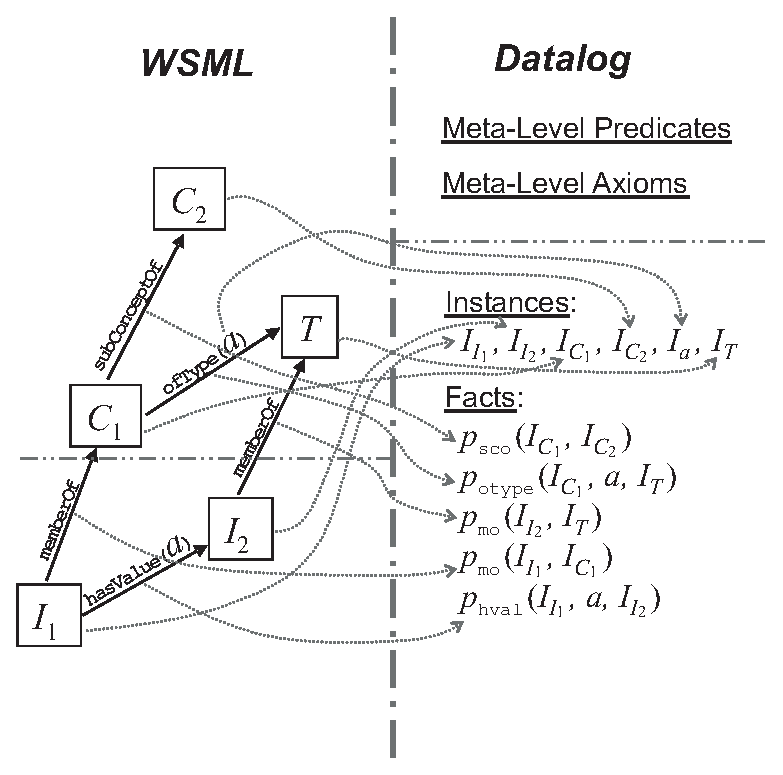
\includegraphics[width=8cm]{figures/meta}
        \centering
    \caption{Meta-level predicates and axioms for realising the WSML semantics. \label{fig:meta}}
\end{figure}

% -- old table for meta-level predicates + meta-level axioms
%\def\filler{\phantom{l}}
%\begin{table}[tb]\label{tab:meta-level}\centering
%\begin{tabular}{|l|l|}
%  \hline
%  \multicolumn{2}{|l|}{\emph{Meta-Level Predicates}} \\
%  \filler \begin{small}Predicate\end{small} & \begin{small}WSML construct\end{small} \\
%  \hline
%  \filler $\psco(C_{sub},C_{sup})$ \qquad\qquad & $C_{sub}$ \wsml{subConceptOf} $C_{sup}$ \\
%  \filler $\pmo(I,C)$ & $I$ \wsml{memberOf} $C$ \\
%  \filler $\phval(I,a,V)$ & $I[a$ \wsml{hasValue} $V]$ \\
%  \filler $\pitype(C,a,T)$ & $C[a$ \wsml{impliesType} $T]$ \\
%  \filler $\potype(C,a,T)$ & $C[a$ \wsml{ofType} $T]$ \\
%  \hline\hline
%  \multicolumn{2}{|l|}{\emph{Meta-Level Axioms}} \\
%  \hline
%  \multicolumn{2}{|l|}{\filler $\psco(C_1,C_3) \leftarrow \psco(C_1,C_2) \wedge \psco(C_2,C_3)$} \\
%  \multicolumn{2}{|l|}{\filler $\pmo(I,C_2) \leftarrow \pmo(I,C_1) \wedge \psco(C_1,C_2)$} \\
%%  \multicolumn{2}{|l|}{\filler $\pmo(V,C_2) \leftarrow \pitype(C_1,a,C_2) \wedge \pmo(I,C_1) \wedge \phval(I,a,V)$} \\
%  \multicolumn{2}{|l|}{\filler $\pmo(V,C_2) \leftarrow \pitype(C_1,a,C_2) \wedge \pmo(I,C_1)$} \\
%  \multicolumn{2}{|l|}{\filler \phantom{$\pmo(V,C_2) \leftarrow$} \qquad $\wedge \phval(I,a,V)$} \\
%%  \multicolumn{2}{|l|}{\filler $ \leftarrow \potype(C_1,a,C_2) \wedge \pmo(I,C_1) \wedge \phval(I,a,V) \wedge \neg \pmo(V,C_2)$} \\
%  \multicolumn{2}{|l|}{\filler $ \leftarrow \potype(C_1,a,C_2) \wedge \pmo(I,C_1)$} \\
%  \multicolumn{2}{|l|}{\filler $ \phantom{\leftarrow} \qquad \wedge \phval(I,a,V) \wedge \neg \pmo(V,C_2)$} \\
% \hline
%\end{tabular}
%\caption{Meta-level axioms and predicates for WSML semantics in
%datalog.}
%\end{table}
\begin{table}[tb]\label{tab:meta-level}\centering
\begin{small}
\begin{tabular}{|ll|}
  \hline
  \multicolumn{2}{|l|}{\rule{0cm}{3.2mm}{\normalsize \emph{Meta-Level Axioms}}} \\
  \hline
  (1) & $\psco(C_1,C_3) \leftarrow \psco(C_1,C_2) \wedge \psco(C_2,C_3)$ \\
  (2) & $\pmo(I,C_2) \leftarrow \pmo(I,C_1) \wedge \psco(C_1,C_2)$ \\
  (3) & $\pmo(V,C_2) \leftarrow \pitype(C_1,a,C_2) \wedge \pmo(I,C_1)$ \\
  & \phantom{$\pmo(V,C_2) \leftarrow$} $\wedge \phval(I,a,V)$ \\
  (4) & $\leftarrow \potype(C_1,a,C_2) \wedge \pmo(I,C_1)$ \\
  & \phantom{$\leftarrow$} $\wedge \phval(I,a,V) \wedge \neg \pmo(V,C_2)$ \\
 \hline
\end{tabular}
\end{small} \caption{Meta-level axioms for WSML semantics in
datalog.}
\end{table}

A fixed set \mlaxioms of datalog rules forms the meta-level axioms
which assure that the proper semantics of the WSML language is
maintained. In these axioms, the meta-level predicates are
interrelated according to the semantics of the different language
constructs. Table \ref{tab:meta-level} shows the rules that make
up the meta-level axioms in \mlaxioms. Axiom (1) realizes
transitivity for the WSML \wsml{subConceptOf} construct, while
axiom (2) ensures that an instance of a subconcept is also an
instance of its superconcepts. Axiom (3) realizes the semantics
for the \wsml{implisType} construct for attribute ranges: any
attribute value is concluded to be in the extension of the range
type declared for the attribute. Finally, axiom (4) realizes the
semantics of the \wsml{ofType} construct by a constraint that is
violated whenever an attribute value cannot be concluded to be in
the extension of the declared range type.

\subsection{Mapping WSML Reasoning Tasks to Datalog Querying}
-- describe how to realise WSML satisfiability and entailment through datalog querying \\
-- -- characterize the KB (datalog program) on which reasoning is performed with the different facts and rules  \\
-- -- show how the WSML reasoning tasks are mapped to datalog queries (KB sat., entailment and conjunctive query answering) \\

To perform reasoning over the original WSML ontology $O$ with an
underlying datalog inference engine, a datalog program
\begin{displaymath}
    P_O = \mlaxioms \cup \tau(O)
\end{displaymath}
is build up, consisting of the meta-level axioms togeter with the
transformed ontology. The different WSML reasoning tasks are then
realized by performing datalog queries on $P_O$, as follows.
\begin{small}
\begin{tabular}{|l|l|}
  \hline
  $O$ is satisfiable & $(P_O, ?\textit{dummyQuery}) \rightarrow true$ \\
  $O \models \phi_g$ & $(P_O, ?\phi_g) \rightarrow true$ \\
  $\{\vec{X} : O \models Q(\vec{X})\}$ & $\{\vec{X} : (P_O, ?Q(\vec{X}) \rightarrow true)\}$ \\
 \hline
\end{tabular}
\end{small}

( $\phi_g$ : ground fact ; $\vec{X}$ : variable binding )


\subsection{Realising Datatype Reasoning}
-- describe how reasoning with datatypes is realised
